\section{Coriander}
\label{sec:coriander}

\begin{spice}\label{spice:coriander}
\textsc{Coriander} \hfill \href{https://powo.science.kew.org/taxon/840760-1}{POWO} \\
\textbf{English:} \textit{coriander}; \textit{cilantro; Chinese parsley}. 
\textbf{Arabic:} {\arabicfont{كزبرة}} \textit{kuzbara}. 
\textbf{Chinese:} {\tc{芫荽}} \textit{yán​sui} [lilac-coriander]. 
\textbf{Hungarian:} \textit{koriander}; \textit{cigánypetrezselyem} [gipsy-parsley].  \\
\noindent{\color{black}\rule[0.5ex]{\linewidth}{.5pt}}
\begin{tabular}{@{}p{0.25\linewidth}@{}p{0.75\linewidth}@{}}
Plant species: & \taxonn{Coriandrum sativum}{L.} \\
Family: & \textit{Apiaceae} \\
part used: & fruit; leaf \\
Region of origin: & Mediterranean; W. Asia; India; SW As \\
Cultivated in: & Argentina; India; Morocco; Romania; Spain; Yugoslavia \\
Color: & light yellow \\
\end{tabular}
\end{spice}

% \begin{figure}[!ht]
% 	\vspace{-4ex}
% 	\centering
% 	\subfloat[\centering a]{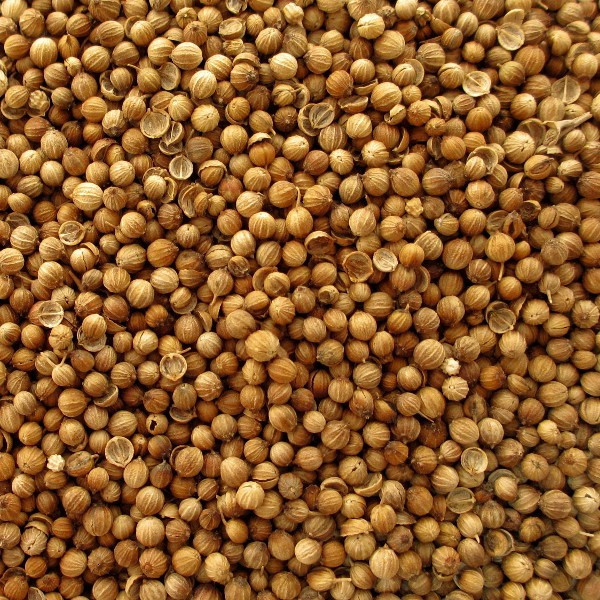
\includegraphics[width=0.3\linewidth]{imgs/spices/coriander-1.jpg}}
% 	\hfill
% 	\subfloat[\centering b]{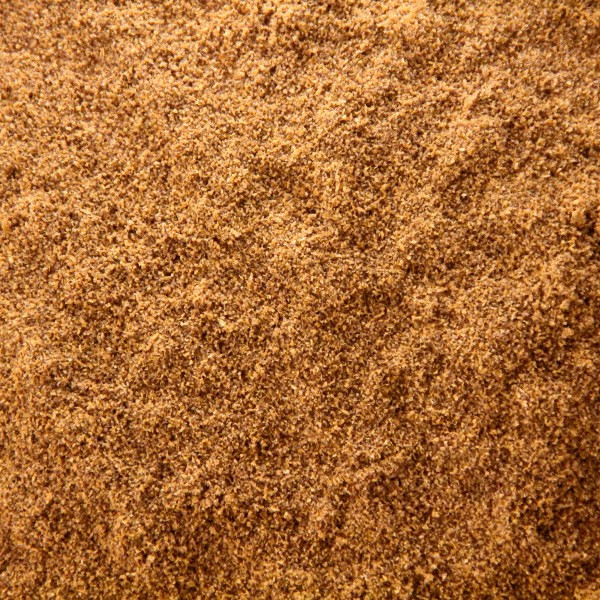
\includegraphics[width=0.3\linewidth]{imgs/spices/coriander-2.jpg}}
% % 	\hfill
% % 	\subfloat[\centering c]{\includegraphics[width=0.3\linewidth]{imgs/spices/coriander-3.jpg}}
% 	\caption{Coriander \textit{}.}
% 	\label{fig:coriander_imgs}
% \end{figure}

\begin{wrapfigure}{R}{0.33\textwidth}
	\vspace{-\baselineskip}
	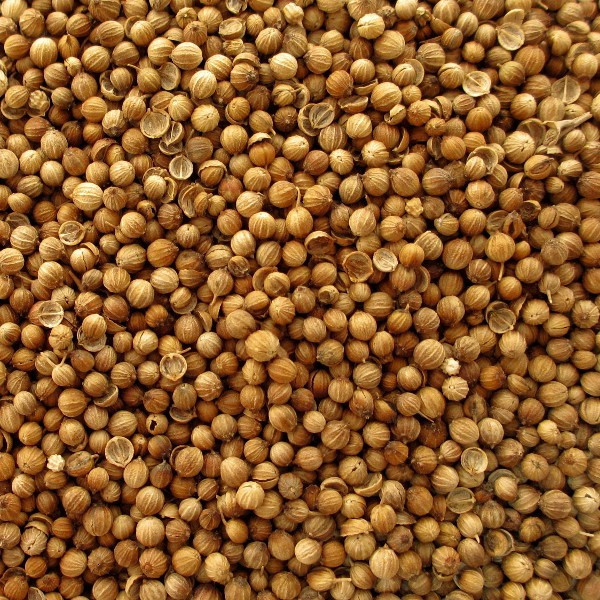
\includegraphics[width=0.33\textwidth]{imgs/spices/coriander-1.jpg}
	\caption{Coriander ``seeds'' (\textit{Coriandrum sativum}).}
	\label{fig:coriander}
\end{wrapfigure}



\subsection{The Botany, Origins, and Cultivation of Coriander}

% Cilantro” should not be confused with “culantro” or “Mexican coriander” (see Eryngium foetidum).

Coriander (\textit{Coriandrum sativum} L.), also known as cilantro and Chinese parsley, is an annual herb originating in Western Asia, with several \glspl{cultivar} consumed around the world. The fresh leaves are used as a culinary herb, popular in Asian, Latin American, and Portuguese cooking, while the dried fruits (``coriander seeds'') are used as a spice, mostly in India, the Middle East, and Europe \autocite{davidson_oxford_2014}. We can essentially talk about two products from one plant, valued for their different culinary properties. The leaves (and the plant itself) are called \textit{cilantro} in the Americas, but also referred to as \textit{fresh coriander} and \textit{coriander greens}. Coriander seeds (often just termed \textit{coriander}) are in fact the plant’s fruits, and ground coriander is a major component of Indian curry powders and pickles. Although nowadays we consider coriander to be a culinary herb and spice and occasional ingredient in liqueurs, its historical role was tending towards a more medicinal one. Moreover, it was used in perfume making, and even in the traditional making of \textit{confetti}\footnote{\url{https://archive.ph/20130414183247/http://www.foodinitaly.org/a-brief-history-of-confetti/}; \url{https://dictionary.cambridge.org/dictionary/italian-english/coriandolo}}.

Coriander is one of the earliest Old World pants used as a condiment \autocite{zohary_domestication_2012}. The exact origin of this ancient crop is hard to define, but the native range is usually set somewhere between the East Mediterranean through the Transcaucasus to Pakistan. We do not know for sure when the species reached the Indian subcontinent \autocite{prance_cultural_2005}, where it enjoys widespread popularity. Coriander and its cultivars have been slowly spread and introduced to most places in Eurasia and grows almost globally in both wild and cultivated forms for thousands of years now.\footnote{For more details on the plant’s distribution, please refer to the Plants of the World Online (POWO) database at: \url{https://powo.science.kew.org/taxon/840760-1\#distribution-map}. Retrieved March 10, 2022.} \textit{Sativum} (Latin for `sown, planted') in the binomial name is a good indicator of this as well.

Coriander and its use have been documented in antiquity, but linguistic and archaeological evidence points to an even longer history. \textcite[163]{zohary_domestication_2012} gives a detailed list of archeobotanical findings, the oldest one of which dates to roughly eight thousand years ago, found in what is today Israel and Palestine. Coriander was also found in Egypt; remnants of desiccated coriander mericarps in Tutankhamun’s tomb (died 1323 BC) are proof for trade or cultivation by the ancient Egyptians \autocite{zohary_domestication_2012}. We know from the Ebers Papyrus – written around 1550 BC, considered amongst the oldest extant medical documents in the world – that the Egyptians used coriander in their medicinal practices \autocite{prance_cultural_2005}. An herbal remedy for headache from these ancient papyri is as follows:

\begin{quote}
\textsc{``Another remedy which the Goddess Isis prepared for the God Ra to drive out the pains that are in his head!}

\smallskip
Berry-of-the-Coriander---I\\
Berry-of-the-Poppy-plant---I\\
Wormwood---I\\
Berry-of-the-sames-plant---I\\
Berry-of-the-Juniper-plant---I\\
Honey---I
\smallskip

Make into one, mix with Honey, and smear therewith in order to make him well forthwith. When this remedy is used by him against all illnesses in the head and all sufferings and evils of any sort, he will instantly become well.'' \textcite[40]{bryan_papyrus_1930}
\end{quote}

Coriander was familiar to the Bronze Age Greeks as well, recorded on Linear B tablets from as early as 2000 BC. According to \textcite{chadwick_mycenaean_1976}, coriander -- reconstructed as \textit{koriadnon} -- must have been grown in both Mycenae and Knossos (on Crete) in considerable amounts, since the epigraphs refer to vast quantities. A tablet found in Pylos for example mentions 576 liters of coriander given to a perfume-maker. Later in antiquity, ancient Greek physicians Hippocrates and Dioscorides mentioned the medicinal properties of coriander, around 400 \textsc{bc} and 65 \textsc{ad}, respectively. Coriander was introduced to England by the Romans, and in 812 Charlemagne ordered its subjects to grow it on the farms of the Holy Roman Empire \autocite{prance_cultural_2005}. It was also one of the first herbs to be introduced to the American colonies, by 1670 it was found in Massachusetts. Due to their relative abundance and widespread distribution, coriander seeds never became a pricey commodity during the spice trade, and as an herb the value is in the freshness of the leaves: it is best when used locally. Nevertheless, the coriander seed world trade total value was at US\$192 million in 2019.\footnote{Data from OEC \url{https://oec.world/en/profile/hs92/coriander-seeds}. Retrieved March 10, 2022.}

\subsection{The History of Coriander}

\subsection{The Names of Coriander}

The word \textit{coriander} entered English in the 14th century via Old French \textit{coriandre}, from Latin \textit{coriandrum}. The Latin word is a borrowing from Greek \textit{koriannon}, a variant of \textit{koriandron}, of uncertain etymology. A shortened version of \textit{korion} also exists, among others. It is often repeated in both popular and scientific literature that the name of coriander comes from the Greek word \textit{koris} `bug, bedbug' (\textit{Cimex lectularius}), for its strong smell of the unripe fruit or the foliage \autocite[cf.][]{harper_coriander_nodate}. According to most contemporary writers, this idea is first promoted by Pliny the Elder (AD 23/24–79), some even purporting that Pliny named the plant after the stinking bug \autocite{oconnell_book_2016, cumo_encyclopedia_2013, prance_cultural_2005} (((O’Connell, 2016, p. 87; Cumo, 2013, p. 318-319; Prance \& Nesbitt, 2005, p. 152))). Pliny mentions coriander multiple times in remedies, stating that the best quality comes from Egypt. However, his monumental work, the \textit{Natural History} \autocite{pliny_the_elder_natural_1855} does not contain any statement of referring to bugs or the name, regarding coriander. The bedbug connection is not often discussed by lexicographers, and dictionaries generally do not endorse it (except \textit{Merriem-Webster's Unabridged}). It seems to be a sort of false etymologization, taken for granted and copied for centuries, reaching as far as a statement in \textit{Encyclopedia Britannica} (1911), although not without reason.

Coriander contains the same aldehydes a stink bug (\textit{Halyomorpha halys}) does, in fact the odor of the stink bug is often likened to that of coriander and (McGee, 2010), and a bed bug infestation reportedly has a similar olfactory experience \autocite{davidson_oxford_2014}. One of the reasons for coriander’s divisive nature is that not all of us perceive these chemicals the same way. Opposing opinions on the smell and benefits of it go back to the Middle Ages, arguments or giants, such as Galen (129--216) and Ibn Sīnā (c. 980--1037) for and against it were reported hundreds of years later \autocite[cf.][]{parkinson_theatrum_1640}. The hatred is so strong from some people, that a series of websites and social media groups are dedicated to it today, under slogans to the effect of “I HATE CILANTRO!” — plus, the term \emph{cilantrophobe} exists. All this has to do with our predisposed genetic differences in perceiving its sensory qualities, and some sources report on Europeans’ (i.e., non-traditional coriander consumers) strong aversive reactions \autocite{eriksson_genetic_2012}. It is also to be noted that the fruits of coriander slightly resemble the appearance of a bedbug as well, and we can speculate that this has also strengthened the connection. Anthropologist \textcite{leach_rehabilitating_2001} retraced the hateful remarks to French and English garden manuals from around the 1600s.
Consulting the Google Books Ngram Viewer \autocite{michel_quantitative_2011}, the first claim of coriander’s name deriving from \textit{koris} in English is from 1640, in John Parkinson’s paramount \textit{Theatrum Botanicum} \autocite[918-919]{parkinson_theatrum_1640}. Other botanists before him also rushed to mention coriander’s stinking character, although not connecting it with the derivation of its name. These include John Gerard in his 1597 \textit{The Herball, or Generall Historie of Plantes} (p. 859) – who mostly plagiarised the Flemish father of botany, Rembert Dodoens and his 1586 work \textit{A nievve herball, or, Historie of plantes} (p. 313), calling it a “very stinking herbe”. In the following centuries both British and American botanists perpetuated this putative word origin. The Mycenaean Greek forms written in Linear B are recorded as ko-ri-ja-do-no /koriʰadnon/ and ko-ri-a2-da-na /korihadna/. \textcite[754]{beekes_etymological_2010} suggest a pre-Greek origin, citing the -dn- cluster, and dismisses both the folk etymologization by \textcite{frisk_griechisches_2021} Frisk (1960/2021) and a possible connection to Akkadian huri’ānu `coriander' proposed by \textcite{szemerenyi_review_1971}. It is more likely then, that those who already disliked coriander (in this case, 16--17\textss{th}-century European botanists) played on the koris-korion link, and arbitrarily conformed the explanation of its name for some personal justification.
Coriander’s synonym, cilantro, is a doublet of coriander. It comes via Spanish culantro from the Late Latin coliandrum a variant of the classical coriandrum. The name cilantro entered English usage relatively late in 1907 \autocite{harper_coriander_nodate} and it usually refers to the fresh leaves people use as garnish. Its use is restricted to North and Latin America, mainly due to the herb’s rise in popularity with the emergence of Mexican cuisine in the United States, bringing the word cilantro with it. (Culantro now is used for an indigenous Latin American herb (\textit{Eryngium foetidum}), also known as long coriander.)

As for the alternative name Chinese parsley, it refers to the leaves as well, never used to the seeds. Some authors and even authoritative encyclopedias presume that the name Chinese parsley is used in China/the Orient, which is a rather silly assumption, since geographic designations are not likely epithets to be used internally \autocite[cf.][]{davidson_oxford_2014, oconnell_book_2016}. The notion to relate coriander to some type of parsley is not far-fetched, the leaves look very similar to other herbs in the \textit{Apiaceae} family (parsley, dill, anise, fennel, etc.). Back to the term Chinese parsley, it apparently emerged in New York at the turn of the century. The phrase first appears in an 1832 United States court document, listing the items of a Chinese grocer, and later in an 1854 work titled \textit{The Transactions of the Royal Hawaiian Agricultural Society}, both without explanation. The first truly interesting story featuring Chinese parsley was an article in Frank Leslie's Popular Monthly, Volume 35 from 1893. The article, A celestial farm on Long Island, introduces how Chinese immigrants have set up farms in the Astoria neighborhood of Queens, in New York City \autocite{seitz_celestial_1893} . The article also contains illustrations, the prices for Chinese vegetables at the time, and identifies Chinese parsley as ``yen sai''\footnote{芫荽 \textit{yán sui}} in Chinese. Hence, it seems plausible that New Yorkers familiarized themselves with the herb from these Chinese farms and this is how the name gained some popularity.



\subsubsection{English}

\begin{etymology}\label{ety:coriander}
English \textit{coriander}
< Old French \textit{coriandre}
< Latin \textit{coriandrum}
< Ancient Greek \textit{korīannon;-dron}\footnote{; }
\end{etymology}

\begin{table}[!ht]
\centering
\begin{tabularx}{\textwidth}{@{}l>{\itshape \small}lL>{\small}l@{}}
\toprule
\textbf{\#} & \multicolumn{1}{l}{\textbf{Species}} & \multicolumn{1}{l}{\textbf{Name}} & \multicolumn{1}{l}{\textbf{Source}} \\
\midrule
1	& Coriandrum sativum	& Chinese parsley	& \textcite{van_wyk_culinary_2014} \\
2	& Coriandrum sativum	& cilantro	& \textcite{van_wyk_culinary_2014} \\
3	& Coriandrum sativum	& coliander	& \textcite{oed} \\
\textbf{4}	& \textbf{Coriandrum sativum}	& \textbf{coriander}	& \textbf{\textcite{van_wyk_culinary_2014}} \\
5	& Coriandrum sativum	& coriander-seed	& \textcite{oed} \\
6	& Coriandrum sativum	& dhania	& \textcite{oed} \\
\bottomrule
\end{tabularx}
\caption{Various names for coriander in English.}
\label{table:names_coriander_en}
\end{table}



\subsubsection{Arabic}

\begin{table}[!ht]
    \caption{Various names for coriander in Arabic.}
\centering
\begin{tabularx}{\textwidth}{@{}l>{\itshape \small}lr>{\itshape}lL>{\small}l@{}}
\toprule
\textbf{\#} & \multicolumn{1}{l}{\textbf{Species}} & \multicolumn{1}{l}{\textbf{Name}} & \multicolumn{1}{l}{\textbf{Tr.}} & \multicolumn{1}{l}{\textbf{Gloss}} & \multicolumn{1}{l}{\textbf{Source}} \\
\midrule
\textbf{1}	& \textbf{Coriandrum sativum}	& \textbf{كزبرة}	& \textbf{kuzbara}	& \textbf{}	& \textbf{\textcite{wehr_dictionary_1976}} \\
\bottomrule
\end{tabularx}
\label{table:names_coriander_ar}
\end{table}



\subsubsection{Chinese}

\begin{table}[!ht]
\centering
\begin{tabularx}{\textwidth}{@{}l>{\itshape \small}ll>{\itshape}lL>{\small}l@{}}
\toprule
\textbf{\#} & \multicolumn{1}{l}{\textbf{Species}} & \multicolumn{1}{l}{\textbf{Name}} & \multicolumn{1}{l}{\textbf{Tr.}} & \multicolumn{1}{l}{\textbf{Gloss}} & \multicolumn{1}{l}{\textbf{Source}} \\
\midrule
1	& Coriandrum sativum	& \traditionalchinesefont{胡荽}	& húsuī	& barbarian-coriander	& \textcite{laufer_sino-iranica_1919} \\
2	& Coriandrum sativum	& \traditionalchinesefont{香菜}	& xiāngcài	& fragrant-vegetable	& \textcite{hu_food_2005} \\
3	& Coriandrum sativum	& \traditionalchinesefont{香茜}	& xiāngqiàn	& fragrant-madder	& \textcite{wikipedia} \\
4	& Coriandrum sativum	& \traditionalchinesefont{芫茜}	& yánqiàn	& lilac-madder	& \textcite{wikipedia} \\
\textbf{5}	& \textbf{Coriandrum sativum}	& \textbf{\traditionalchinesefont{芫荽}}	& \textbf{yánsuī}	& \textbf{lilac-coriander}	& \textbf{\textcite{hu_food_2005}} \\
\bottomrule
\end{tabularx}
\caption{Various names for coriander in Chinese.}
\label{table:names_coriander_zh}
\end{table}



\subsubsection{Summary}

\begin{table}[!ht]
    \caption{Conventionalized names for coriander in English, Arabic, and Chinese, found in dictionaries.}
\centering
\begin{tabularx}{\textwidth}{@{}ll>{\itshape}lLl>{\small}l@{}}
\toprule
\textbf{\#} & \textbf{Language} & \multicolumn{1}{l}{\textbf{Term}} & \textbf{Gloss} & \textbf{Loan} & \multicolumn{1}{l}{\textbf{Source}} \\
\midrule
1	& English	& Chinese parsley	& 	& no	& \textcite{oed} \\
2	& English	& cilantro	& 	& yes	& \textcite{oed} \\
3	& English	& coliander	& 	& yes	& \textcite{oed} \\
4	& English	& coriander	& 	& yes	& \textcite{oed} \\
5	& English	& coriander-seed	& 	& no	& \textcite{oed} \\
6	& English	& dhania	& 	& yes	& \textcite{oed} \\
\midrule
1	& Arabic	& kuzbara	& 	& yes	& \textcite{wehr_dictionary_1976} \\
\midrule
1	& Chinese	& húsuī	& barbarian-coriander	& yes	& \textcite{defrancis_abc_2003} \\
2	& Chinese	& xiāngcài	& fragrant-vegetable	& no	& \textcite{mdbg} \\
3	& Chinese	& yánsuī	& lilac-coriander	& no	& \textcite{mdbg} \\
\bottomrule
\end{tabularx}
\label{table:names_coriander}
\end{table}



% English,coriander
% Old French,coriandre
% Latin,coriandrum
% Ancient Greek,korīannon;-dron

% EE:
% the plant Coriandrum sativum. XIV. — (O)F. coriandre — L. coriandrum — Gr. korīannon, -dron.

% OE:
% coriander (n.)

% popular name of an umbelliferous plant (Coriandrum sativum) with a seed-like aromatic fruit, late 14c., coriaundre, from Old French coriandre (14c.), from Latin coriandrum, from Greek koriannon, often said by botanists to be related to koris "bedbug" from the bad smell of the unripe fruit, or perhaps it is a non-Indo-European word conformed to the Greek insect name.
% Entries linking to coriander
% cilantro (n.)
% alternative name for coriander, by 1907, from Spanish cilantro, variant of culantro, from Latin coriandrum "coriander" (see coriander).

% MW:
% Middle English coriandre, from Old French, from Latin coriandrum, from Greek koriandron, koriannon, from koris bedbug; from its odor — more at coreidae

% First Known Use: 14th century (sense 1)

% AH:
% [Middle English coriandre, from Old French, from Latin coriandrum, from Greek koriandron.]

% WK:
% From Middle English coriandre, from Anglo-Norman coriandre, from Old French corïandre, from Latin coriandrum, from Ancient Greek κορίανδρον (koríandron), of uncertain origin.

% Compare Ancient Greek κορίαννον (koríannon), κορίαμβλον (koríamblon), Mycenaean Greek ���������� (ko-ri-ha-da-na), ���������� (ko-ri-ja-da-na), ���������� (ko-ri-ja-do-no), ���������� (ko-ri-jo-da-na), and Akkadian �������� (úḫurium).

% Beekes supposes that cluster -dn- implies a Pre-Greek word, and hypothesizes that *koriaⁿdro- may have dissimilated to *koriaⁿdno-.

% Doublet of cilantro. 

